\documentclass[12pt,a4paper]{report}

% Packages
\usepackage[utf8]{inputenc}
\usepackage{amsmath, amssymb, amsfonts}
\usepackage{graphicx}
\usepackage{subcaption}
\usepackage{algorithm2e}
\usepackage{fancyhdr}
\usepackage{geometry}
\usepackage[colorlinks=false, pdfborder={0 0 0}]{hyperref}
\usepackage{lipsum}
\usepackage{natbib}
\usepackage{amsthm}
\usepackage{tikz}
\usepackage{ragged2e}
\usepackage{setspace}
\usepackage{float} % for [H] placement

% Geometry and Page Style
\geometry{left=3cm, right=3cm, top=2.5cm, bottom=2.5cm}
\pagestyle{fancy}
\fancyhf{}
\rhead{Technical Writing using LaTeX}
\lfoot{Rajeev Institute of Technology}
\rfoot{\thepage}

% Line Spacing
\onehalfspacing

% Theorem Styles
\newtheorem{theorem}{Theorem}[chapter]
\newtheorem{corollary}{Corollary}[theorem]
\newtheorem{lemma}[theorem]{Lemma}
\newtheorem{definition}{Definition}[section]

\begin{document}

% Title Page
\begin{titlepage}
    \centering
    {\scshape\LARGE Your Institute Name \par}
    \vspace{1cm}
    {\scshape\Large Technical Writing using LaTeX\par}
    \vspace{1.5cm}
    {\huge\bfseries Comprehensive Report\par}
    \vspace{2cm}
    {\Large\itshape Hemanth S.P\par}
    \vfill
    Supervisor: \textbf{Supervisor Name}

    \vfill

    {\large \today\par}
\end{titlepage}

% Certificate Page
\chapter*{Certificate}
\thispagestyle{empty}
\begin{center}
    \textbf{\large Visvesvaraya Technological University}\\
    \textbf{\small JnanaSangama, BELAGAVI - 590018}\\
    \vspace{0.5cm}
    \textbf{\small DEPARTMENT OF COMPUTER SCIENCE AND ENGINEERING}\\
    \vspace{0.5cm}
    \textbf{\large CERTIFICATE}
\end{center}
\vspace{0.5cm}
\justify
This is to certify that Mr./Ms. \underline{Hemanth S.P}{\hspace{0.1cm}} has successfully completed the project titled \textbf{"Technical Writing using LaTeX"} under the guidance of \textbf{Supervisor Name} in partial fulfillment of the requirements for the award of the degree of Bachelor of Engineering in Computer Science and Engineering of Visvesvaraya Technological University, Belagavi, Karnataka.
\vspace{1cm}

\begin{flushleft}
\textbf{Signature of Guide} \hfill \textbf{Signature of HOD} \hfill \textbf{Signature of Principal}
\end{flushleft}

\newpage

% Abstract
\begin{abstract}
\justify
This report demonstrates the importance and usage of LaTeX in academic and technical documentation. LaTeX, known for its typesetting quality, is widely used for producing scientific and mathematical documents due to its powerful handling of formulas, bibliographies, and structured content.

This work includes examples across 11 chapters, explaining each concept through code and rendered output. Chapters explore document design, equation typesetting, theorem environments, tables and graphics handling, algorithms using pseudo-code, and bibliographic citations. The final sections emphasize how all these elements synergize in producing professional-quality reports and theses.

The goal is to familiarize students with LaTeX basics and advanced features to create well-organized and publish-ready documents.
\end{abstract}

\newpage

% Table of Contents
\tableofcontents
\newpage

% Chapter 1: Introduction
\chapter{Introduction}
\section{Simple Document}
\justify
\lipsum[1-3]
LaTeX provides a robust solution for creating high-quality documents. A typical LaTeX document consists of a preamble (for setting document class and loading packages) and the content body. 
LaTeX enforces structure through sections, chapters, and logical divisions, which is essential in academic writing.

\section{Importance of LaTeX}
\justify
LaTeX separates content from presentation. This allows writers to focus on the document's logical flow while LaTeX handles formatting. Unlike WYSIWYG word processors, LaTeX encourages structured and clean documents.

\lipsum[4]

% Chapter 2: Abstract/Summary
\chapter{Abstract/Summary}
\section{Sample Abstract}
\justify
\lipsum[5-6]

% Chapter 3: Title and Certificate Pages
\chapter{Title and Certificate Pages}
\section{Title Page}
\justify
The title page is structured using the \texttt{titlepage} environment. It includes the university name, report title, author, supervisor, and submission date. This sets the first impression of your report.

\section{Certificate Page}
\justify
The certificate authenticates the student’s work and is signed by the guide, HOD, and principal. It confirms the submission of original work under proper guidance.

\lipsum[7]

% Chapter 4: Tables
\chapter{Tables}
\section{Student Marks Table}
\begin{table}[H]
\centering
\begin{tabular}{|c|c|c|c|c|c|}
\hline
Sl & USN & Student Name & Subject1 & Subject2 & Subject3 \\
\hline
1 & 4XX22XX001 & Name1 & 89 & 60 & 90 \\
2 & 4XX22XX002 & Name2 & 78 & 45 & 98 \\
3 & 4XX22XX003 & Name3 & 67 & 55 & 59 \\
\hline
\end{tabular}
\caption{Student Marks}
\end{table}

\justify
Tables in LaTeX are structured using the \texttt{tabular} environment. Borders, alignment, and formatting options give full control over presentation.

% Chapter 5: Graphics
\chapter{Graphics}
\section{Side-by-Side Images}
\begin{figure}[H]
\centering
\begin{subfigure}{0.45\textwidth}
    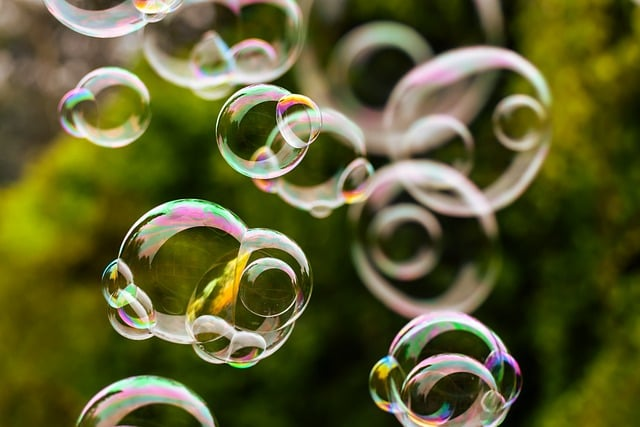
\includegraphics[width=\linewidth]{image1.jpg}
    \caption{Image 1}
\end{subfigure}
\hfill
\begin{subfigure}{0.45\textwidth}
    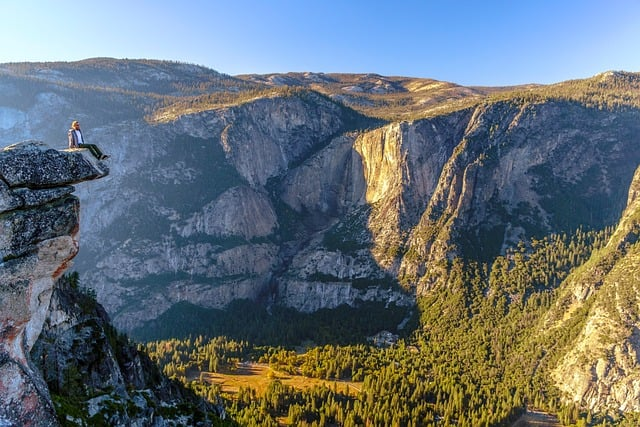
\includegraphics[width=\linewidth]{image2.jpg}
    \caption{Image 2}
\end{subfigure}
\caption{Side-by-side Images}
\end{figure}

\justify
The \texttt{graphicx} package enables image inclusion and manipulation. Using \texttt{subcaption}, we can arrange multiple images neatly side-by-side.

% Chapter 6: Mathematical Equations
\chapter{Mathematical Equations}
\section{Einstein's Mass-Energy Equivalence}
\begin{equation}
E = mc^2
\end{equation}

\section{Quadratic Formula}
\begin{equation}
x = \frac{-b \pm \sqrt{b^2 - 4ac}}{2a}
\end{equation}

\justify
LaTeX excels at rendering complex equations using the \texttt{amsmath} package.

% Chapter 7: Theorems and Definitions
\chapter{Theorems and Definitions}
\section{Sample Theorem}
\begin{theorem}[Accessible Pointed Graph]
\justify
Consider an XML database D and a twig query q with only ancestor, descendant relationships in branching edges. The worst-case I/O complexity is decided by the number of holistic nodes in the path algebra.
\end{theorem}

\section{Sample Corollary}
\begin{corollary}
Every valid subtree extracted from an accessible pointed graph satisfies the uniqueness constraint in XML.
\end{corollary}

\section{Sample Lemma}
\begin{lemma}
Every connected acyclic graph has at least one leaf node.
\end{lemma}

\section{Sample Definition}
\begin{definition}
A tree is a connected graph without cycles.
\end{definition}

% Chapter 8: Citations and Bibliography
\chapter{Citations and Bibliography}
\section{Sample Citations}
\justify
As discussed in \cite{latexcompanion}, LaTeX provides a high-quality typesetting system. Further details can be found in \cite{knuth1984texbook} and \cite{lamport1994latex}.

\section{Bibliography}
\bibliographystyle{plain}
\bibliography{references}

% Chapter 9: Algorithms
\chapter{Algorithms}
\section{Sample Algorithm}
\begin{algorithm}[H]
\SetAlgoLined
\KwResult{Factorial of n}
Initialize result $\gets$ 1\;
\For{$i \gets 2$ \KwTo $n$}{
    result $\gets$ result $\times$ i\;
}
\Return{result}
\caption{Factorial Calculation}
\end{algorithm}

% Chapter 10: TikZ Diagrams
\chapter{TikZ Diagrams}
\section{Sample Tree Diagram}
\begin{center}
\begin{tikzpicture}[sibling distance=10em,
  every node/.style = {shape=rectangle, draw, align=center}]
  \node {Root}
    child { node {Child 1}
      child { node {Grandchild 1} }
      child { node {Grandchild 2} }
    }
    child { node {Child 2}
      child { node {Grandchild 3} }
      child { node {Grandchild 4} }
    };
\end{tikzpicture}
\end{center}

% Chapter 11: Conclusion
\chapter{Conclusion}
\justify
This report offered a hands-on overview of LaTeX. By breaking down individual features across separate chapters, readers gain a modular understanding of its components. Students are encouraged to experiment and expand each section, developing custom commands and styles as needed.

The power of LaTeX lies in its automation, scalability, and precision—making it a valuable tool for students, researchers, and authors.

\lipsum[10]

\end{document}
